\documentclass[a4paper]{article}
\usepackage{geometry}
\usepackage{algorithm}
\usepackage{algorithmic}
\usepackage{amsmath}
\usepackage{amssymb}
\usepackage{amsthm}
\usepackage{graphicx}
\usepackage{epstopdf}
\usepackage{subfigure}
%\usepackage{subcaption}
\usepackage{indentfirst}
\usepackage{cite}

\title{A Variant of the Line Sweep Algorithm with User-defined Uncertainty Quantification}
\author{Zhixuan Li}

\newtheorem{prop}{Proposition}
\newtheorem{definition}{Definition}

\begin{document}
\maketitle

\section{Introduction}
Computing the intersections of a set of line segments
is one fundamental routine in computational geometry.
The line sweep algorithm \cite{CG} is an efficient scheme
for solving this problem.
In this article, we introduce a variant of the line sweep algorithm.
While preserving the efficient nature,
our algorithm is amenable to float-point errors, 
and is adaptive to problems of all scales by
using a user-defined uncertainty quantification.
In addition, it is capable of computing the incident segments
for each intersection, assuming no precondition on the input.

\section{Algorithm}
Our algorithm accepts a multiset of line segments as input.
The plain version of the line sweep algorithm fails to
deal with cases such as improper intersections and overlapping segments. 
In order to deal with overlapping segments,
we introduce the concept of a \emph{bundle}.
A bundle is an unordered set of segments
that overlaps at the level of the sweep line.
In our algorithm, the status structure $\mathcal{T}$ is designed to be
an ordered set whose elements are bundles.
Accordingly, 
adding segments into $\mathcal{T}$ now
adds to the corresponding bundle,
and intersecting adjacent segments now becomes
intersecting adjacent bundles, etc.

%\begin{figure}[htb]
%  \centering
%  \includegraphics[width=0.3\textwidth]{t1.eps}
%  \caption{An illustration of the concept \emph{bundle}. }
%\end{figure}

\newcommand{\Lhat}{\hat{L}}
\newcommand{\Uhat}{\hat{U}}
\newcommand{\Chat}{\hat{C}}

\begin{algorithm}[htbp]
  \caption{findIntersections(S)}
  \label{alg:fi}
  \begin{algorithmic}[1]
    \renewcommand{\algorithmicrequire}{\textbf{Input : }}
    \REQUIRE $S = \{s_1,\cdots,s_n\}$ is a multiset of line segments
    that may contain overlapping segments.
    \renewcommand{\algorithmicrequire}{\textbf{Precondition : }}
    % \REQUIRE The overlie of any two segments does not overlap another segment.
    \REQUIRE None
    \renewcommand{\algorithmicensure}{\textbf{Output : }}
    \ENSURE $\Omega$ is the point set of the intersections.
    inc($p$) is the segments incident to $p$, $\forall p \in \Omega$.
    \renewcommand{\algorithmicensure}{\textbf{Postcondition : }}
    \ENSURE Each intersection point with its incident segments is reported.
    
    For overlapping segments, endpoints of the overlie are reported.
    
    \STATE Empty the priority queue $\mathcal{Q}$.
    Let all the endpoints of the segments in $S$ enqueue.

    \STATE For each endpoint in $\mathcal{Q}$,
    initialize $L(p), U(p)$ accordingly, 
    where $L(p)$ is the set of the segments whose upper endpoint is $p$,
    and $U(p)$ likewise.
    Initialize $C(p)$ to empty.

    \STATE Empty the status structure $\mathcal{T}$.
    \STATE 

    \WHILE{$\mathcal{Q}$ is not empty}

      \STATE Pop the top event in $\mathcal{Q}$, denoted as $p$

      \IF{$L(p) \cup C(p) = \emptyset$}
      \STATE Pick an arbitrary segment from $U(p)$, say $s'$. 
      \STATE $B'$ = \textbf{addToStatus}($\mathcal{Q},\mathcal{T},s'$). 
      \STATE \textbf{findNewEvent}($\mathcal{Q},\{s'\}$,pred($B'$),$p$). 
      \STATE \textbf{findNewEvent}($\mathcal{Q},\{s'\}$,succ($B'$),$p$). 
      \STATE /* pred($B'$), succ($B'$) stand for the predecessor and the succesor
      of bundle $B'$ in $\mathcal{T}$. */

      \STATE Remove $s'$ from $\mathcal{T}$.
      \ENDIF
      \label{alg:incdone}

      \STATE Remove $L(p) \cup C(p)$ from $\mathcal{T}$.

      \STATE For each segment $s \in C(p) \cup U(p)$
      do \textbf{addToStatus}($\mathcal{Q},\mathcal{T},s$). 
      
      \IF{$C(p) \cup U(p) = \emptyset$}
      \label{alg:testadjbeg}
      \STATE Let $B'$ be the successor of the rightmost bundle
      among $L(p)$ before deletetion. 
      \STATE \textbf{findNewEvent}($\mathcal{Q},B'$,pred($B'$),$p$). 
      \ELSE
      \STATE Let $B_l$ be the leftmost bundle among $U(p) \cup C(p)$,
      and $B_r$ be the rightmost one. 
      \STATE \textbf{findNewEvent}($\mathcal{Q},B_l$,pred($B_l$),$p$). 
      \STATE \textbf{findNewEvent}($\mathcal{Q},B_r$,succ($B_r$),$p$). 
      \ENDIF
      \label{alg:testadjend}

      \STATE
      \IF{$\vert L(p) \cup C(p) \cup U(p)\vert >= 2$}
      \STATE $\Omega \leftarrow \Omega \cup \{p\}$. 
      \STATE $\text{inc}(p) \leftarrow L(p) \cup C(p) \cup U(p)$. 
      \ENDIF
     
    \ENDWHILE
    
  \end{algorithmic}
\end{algorithm}

\begin{algorithm}[htbp]
  \caption{findNewEvent($\mathcal{Q},B_l$,$B_r$,$p$)}
  \label{alg:fne}
  \begin{algorithmic}[1]
    \renewcommand{\algorithmicensure}{\textbf{Side effect : }}
    \ENSURE $\mathcal{Q}$ is modified.
    \FOR{each pair of segments $s_1,s_2$ from $B_l,B_r$ respectively}
    \FOR{each intersection $q$ of $s_1$ and $s_2$}
    \IF{ $p$ equals $q$ or $p$ is prior to $q$}
    \STATE Let $q$ enqueue. 
    \STATE Add $s_1$ to $C(q)$ if $s_1 \notin L(q) \cup U(q)$
    and do the same for $s_2$. 
    \ENDIF
    \ENDFOR
    \ENDFOR
  \end{algorithmic}
\end{algorithm}

% \begin{algorithm}[htbp]
%   \caption{collect($U(p)$)}
%   \label{alg:hd}
%   \begin{algorithmic}[1]
%     \renewcommand{\algorithmicrequire}{\textbf{Precondition : }}
%     \REQUIRE $U(p) \neq \emptyset$
    
%     \STATE Pick any segment from $U(p)$, say $s'$. Add $s'$ to $\mathcal{T}$.
%     Suppose $s'$ belong to the bundle $B'$.
%     \STATE \textbf{findNewEvent}($\{s'\}$,pred($B'$),$p$)
%     \STATE \textbf{findNewEvent}($\{s'\}$,succ($B'$),$p$)
%     \STATE Remove $s'$ from $\mathcal{T}$.
%   \end{algorithmic}
% \end{algorithm}

\begin{algorithm}[htbp]
  \caption{addToStatus($\mathcal{Q},\mathcal{T},s$)}
  \begin{algorithmic}[1]
    \renewcommand{\algorithmicensure}{\textbf{Side effect : }}
    \ENSURE $\mathcal{Q}, \mathcal{T}$ is modified.
    \IF{$s$ belongs to some existing bundle $B$ in $\mathcal{T}$}
    \STATE $B = B \cup \{s\}$. 
    \STATE \textbf{findNewEvent}($\mathcal{Q},\{s\}$,$B \setminus \{s\}$,$p$). 
    \ELSE
    \STATE Create a new bundle $B' = \{s\}$.
    Let $\mathcal{T} = \mathcal{T} \cup \{B'\}$.
    \ENDIF
  \end{algorithmic}
  \label{alg:ats}
\end{algorithm}

\section{Analysis}

\subsection{Correctness}

For any input $S$,
we can choose the slope of the sweep line to be some tiny positive $\delta$
so that no segment in $S$ is parallel to the sweep line.
Algorithmically, this is equivalent to :
(i) using a horizontal sweep line; 
(ii) sorting the event points using their $x$ coordinates as minor keyword
($y$ coordinates as major keyword).
Hence it is safe to assume the input does not contain any horizontal segment.

Before moving on to prove the corrrectness of Algorithm \ref{alg:fi},
we would like to make some comments on the algorithm.
In fact, finding the intersections is done in Line 2, Algorithm \ref{alg:fne}.
The call to Algorithm \ref{alg:fne} happens in three places : 
Line 10-11 in Algorithm \ref{alg:fi}; 
Line 17-24 in Algorithm \ref{alg:fi}; 
and Line 3 in Algorithm \ref{alg:ats}. 
Intuitively speaking,
\begin{itemize}
\item Line 17-24 tests for intersection among each pair of bundles that become newly adjacent.
\item Line 3 in Algorithm \ref{alg:ats} calculates the endpoints of the overlie
  (which is implied by the condition in Line 1 being satisfied).
\item Line 7-13 in Algorithm \ref{alg:fi} deals with a special case
  which will be explained later.
\end{itemize}
In the plain version of the line sweeping algorithm, only the first measure is taken.
The second and the third measure is needed here because we need to deal with degenerate cases.
In the proof of the following Proposition, we argue that these three measures combined
are all we need in order to correctly find out the segments incident to an event point.

\begin{prop}
  Upon the finish of Line \ref{alg:incdone} in Algorithm \ref{alg:fi},
  all segments incident to the current event point $p$ are found.
  \label{prop:segfound}
\end{prop}
\begin{proof}
  Segments that has $p$ as endpoint
  can certainly be found due to the work of Line 3.
  So we focus on showing $C(p)$ contains all the segments that have $p$ in their interior.
  \begin{enumerate}
  \item The conclusion natually holds under the trivial case of $C(p) = \emptyset$.
  \item Since the sweeping line is moving up-down,
    at the moment right before the sweep line reaches the current event point,
    the sweep line intersects with all the bundles in $L(p) \cup C(p)$.
    If $L(p) \cup C(p)$ contributes to two or more bundles,
    then each pair of neighbouring bundles has already been tested in the previous events
    due to the work of Line \ref{alg:testadjbeg}-\ref{alg:testadjend}.
    In this case, $C(p)$ can be correctly found.
  \item Now suppose the contrary, i.e., $L(p) \cup C(p)$ consists of only one bundle.
    Recall that Algorithm \ref{alg:ats} guarantees that inside this bundle,
    each pair of segments is tested against when they are inserted into $\mathcal{T}$.
    So if $L(p)$ is non-empty, say there is some $s' \in L(p)$,
    all segments in $C(p)$ has been tested against $s'$ in the previous events
    (either in the upper event of $s'$ or
    in the upper events of the segments in $C(p)$).
  \item The last possibility is that
    $L(p) \cup C(p)$ consists of only one bundle and $L(p) = \emptyset$.
    However this implies $U(p) \ne \emptyset$ or otherwise, $p$ cannot be an event point.
    Note that the segments in $C(p)$ never have the chance of
    being tested against the segments in $U(p)$,
    so upon the finish of Line 6 $C(p)$ is still empty.
    Line 7 serves as the entering condition for this case,
    and Line 8-13 recovers the true $C(p)$.
  \end{enumerate}
  

%   If $C(p) = \emptyset$, of course $C(p)$ is correctly computed.
% %  so let us further assume $C(p) \ne \emptyset$.
%   Note that Line \ref{alg:testadjbeg}-\ref{alg:testadjend} tests all pairs of bundles
%   that become newly adjacent right below any previous event point.
%   So if $L(p) \cup C(p)$ contains more than 2 bundles,
%   $C(p)$ is also correctly computed.
%   Let us further assume $L(p) \cup C(p)$ contain only one bundle
%   and $C(p) \ne \emptyset$.

%   If $L(p) \ne \emptyset$,
%   suppose among $L(p) \cup C(p)$, $s$ has the lowest upper endpoint. 
%   But when $s$ was added to the current bundle,
%   $s$ was tested against all other segments in this bundle
%   (Algorithm \ref{alg:ats} Line 3)
%   so $C(p)$ is correctly found.

%   Finally if $L(p) = \emptyset$, then $U(p) \neq \emptyset$
%   (otherwise $p$ cannot become an event point).
%   However by the time $p$ is popped,
%   the $C(p)$ bundle is never tested against any bundle in $U(p)$
%   and thus by then $C(p)$ is still empty during the running of the algorithm.
%   Line 8 captures this case and Line 9 recovers $C(p)$.
\end{proof}

\begin{prop}
  All the intersections are reported by Algorithm \ref{alg:fi}.
\end{prop}
\begin{proof}
  By Proposition \ref{prop:segfound} and Line 26-29,
  it suffices to show any intersection has ever been presented in $\mathcal{Q}$.
  
  If $p$ is a proper intersection,
  then slightly above $p$ there exists two (or more) adjacent bundles emitted from $p$.
  Line \ref{alg:testadjbeg}-\ref{alg:testadjend} guarantees that any pair of bundles that become newly adjacent is tested,
  thus $p$ is put enqueued at some moment.
  If $p$ is an improper intersection, $p$ must be an endpoint,
  and it is in $\mathcal{Q}$ from the beginning.
  
\end{proof}

%\begin{figure}[htb]
%  \centering
%  \subfigure[]{
%    \includegraphics[width=0.2\textwidth]{r1.eps}}
%  \subfigure[]{
%    \includegraphics[width=0.2\textwidth]{r2.eps}}
%  \caption{The only two cases that $C(p)$ is recovered by Line 8-12, Algorithm \ref{alg:fi}. }
%  \label{fig:collect}  
%\end{figure}


\subsection{Complexity}
Table \ref{tab:not} is a list of notations we shall use in the complexity analysis.
\begin{table}[htb]
  \centering
  \begin{tabular}{|c|l|}
  \hline
    $S$ & The multiset of segments. \\
    \hline
    $\Omega$ & The set of intersections. \\
    \hline
    $n$ & $\vert S  \vert$, the number of segments.  \\
    \hline
    $I$ & $\vert \Omega \vert$, the number of intersections. \\
    \hline
    $e$ & The total number of event points. \\
    \hline
    $m(p)$ & $\vert L(p) \cup C(p) \cup U(p)  \vert$. \\
    \hline
    $m$ & $\sum_{p} m(p)$ as $p$ ranges over all event points.  \\
    \hline
    $k$ & $\sum_{p \in \Omega} \vert \text{inc}(p) \vert$, the number of output. \\
    \hline
  \end{tabular}
  \caption{Notations.}
  \label{tab:not}
\end{table}

\begin{definition}
  The \emph{bundle size} $\mu(S)$ of a multiset of segments $S$ is
  the maximum number of overlapping segments. 
  In symbol, 
  \begin{equation}
    \mu(S) = \max \left\{ \vert U \vert : U \subset S, 
    \text{the intersection of members of } U \text{is a segment} \right\}. 
  \end{equation}
\end{definition}

% It's straightforward to see that
% \emph{The overlie of any two overlapping segments in $S$ does not overlap another segment}
% implies $\mu(S)=2$.

\newcommand{\bigO}[1]{\mathcal{O}(#1)}

\begin{prop}
  If $\mu(S) = \bigO{1}$,
  Algorithm \ref{alg:fi} takes time $\bigO{m \log n}$.
  \label{prop:tcw}
\end{prop}
\begin{proof}

  % \item
  The initialization in Line 1-2 involves $2n$ times of
    maintenance of balanced-tree (MOB),
    thus it takes $\bigO{n\log n}$. Line 3 takes $\bigO{1}$.
    In each loop, Line 6-14,
    \ref{alg:testadjbeg}-\ref{alg:testadjend} involes
    constant many times of MOB and intersection findings
    because $\mu(S) = \bigO{1}$.
    Hence these lines of code cost $\bigO{e \log n}$ throughout the algorithm.
    In Line 26-29, output to $\Omega$ involves
    at most $2e$ insertions to a linear container
    since event points are sorted, 
    while output to $\text{inc}(p)$ takes $\bigO{k}$.
    Again from $\mu(S) = \bigO{1}$,
    Line 15-16 involes $\bigO{m}$ times of MOB,
    so it takes $\bigO{m \log n}$.


    Up to now we have the estimation of $\bigO{(n+e+m) \log n}$,
    eliminating the insignificant terms.
    But it's easy to see that $n \le m, e \le m$ and the conclusion follows.

\end{proof}

\begin{prop}
  If $\mu(S) = \bigO{1}$,
  Algorithm \ref{alg:fi} takes time $\bigO{(n+I) \log n}$.
  \label{prop:tc}
\end{prop}
\begin{proof}
  We follow the approach of Lemma 2.3 in \cite{CG} to show $m=\bigO{n+I}$.
  
  From now on we interpret $S$ as a planar graph embedded in the plane.
  Let $n_e$ denote the number of edges, and $n_v$ the number of vertices.
  Since $m(p)$ is bounded by $\mu(S)$ times the degree of $p$,
  it follows that $m$ is bounded by $\mu(S)$ times the sum of degrees.
  But every edge adds 2 to the sum of degrees, 
  hence $m$ is bounded by $2 \mu(S) n_e$.
  By \emph{Euler's formula}, $n_e = \bigO{n_v}$.
%
%  Although our algorithm deals with extra degenerate cases, i.e.
%  \begin{itemize}
%  \item one segment intersects the other at the endpoint.
%  \item two segments overlap but endpoints are the only intersections to report.
%  \end{itemize}
%  In either of the above cases, the reported intersections belongs to endpoints.
  By the definition of $I$, we have $n_v \le 2n + I$. 
  Combined with Proposition \ref{prop:tcw}, 
  the time complexity is indeed $\bigO{(n+I) \log n}$.
\end{proof}

\begin{prop}
  Algorithm \ref{alg:fi} consumes $\bigO{n+I}$ space.
\end{prop}
\begin{proof}
  The size of the status structure $\mathcal{T}$ never exceeds $n$.
  By definition the event queue $\mathcal{Q}$ along with
  $L(p),C(p),U(p)$ takes $\bigO{m}$ space.
  From the proof of Proposition \ref{prop:tcw} and \ref{prop:tc}
  we know $\bigO{n+m} = \bigO{n+I}$.
\end{proof}

\section{Test}
%Part of the tests are as in Figure \ref{fig:test}.
%All the tests required by the Question (d) are performed,
%as well as some chanllenging cases.
%Figure \ref{fig:test} is the visualized output of part of the tests.
%For more details, reproduce the results by calling the \textit{testAll}.

% \begin{figure}
%   \centering
%   \subfigure[Page 21 upper]{
%     \includegraphics[width=0.4\textwidth]{../results/testLineInts-2.png}}
%   \subfigure[Overlapping segments]{
%     \includegraphics[width=0.4\textwidth]{../results/testLineInts-5.png}}
%   \subfigure[Horizontal segments and improper intersections]{
%     \includegraphics[width=0.4\textwidth]{../results/testLineInts-4.png}}
%   \subfigure[Identical segments]{
%     \includegraphics[width=0.4\textwidth]{../results/testLineInts-6.png}}
%   \subfigure[Page 23]{
%     \includegraphics[width=0.4\textwidth]{../results/testLineInts-7.png}}
%   \subfigure[Horizontal + overlapping + improper]{
%     \includegraphics[width=0.4\textwidth]{../results/testLineInts-10.png}}
%   \caption{Visualized output of the algorithm}
%   \label{fig:test}
% \end{figure}

\bibliography{ref}
\bibliographystyle{plain}

\end{document}
